% \lipsum[2-3]

\section{Motivation}
\section{Aufgabenstellung}
\section{Zusammenfassung des Projektergebnisse}
\section{Projektvorgehensmodell}
\subsection{Projektorganisation}

\subsubsection{Discord}
\setauthor{Martin Hausleitner}
Unsere primäre Kommunikationsplattform zwischen unserem Team und unseren Diplomarbeit-Betreuern ist Discord.

Da wir in den Sommerferien 2022 mit unserer Arbeit begonnen
haben und zu diesem Zeitpunkt Corona-Regelungen galten,
mussten wir eine Meeting-Plattform finden, die sowohl Video-
als auch Text-Chat ermöglicht. Aufgrund unserer Vertrautheit
mit Discord und der Tatsache, dass es kostenlos ist, fiel
die Entscheidung leicht.

Während unserer Diplomarbeit haben wir über 40 Text-Kanäle erstellt, um alle relevanten Informationen, Notizen und Dokumente zu speichern. Die Meeting-Notizen wurden jedoch auf ClickUp gespeichert.
\subsubsection{ClickUp}
\setauthor{Martin Hausleitner}
Um unser Projekt effizient zu organisieren, nutzen wir nicht nur eine WhatsApp-Gruppe, sondern auch das Projektmanagement-Tool ClickUp. Die Entscheidung für ClickUp fiel uns leicht, da ich persönlich bereits viele Projektmanagement-Programme ausprobiert habe und ClickUp bei meinen letzten Projekten am besten abgeschnitten hat. Zudem ist es sehr intuitiv und einfach zu erlernen, wie auch meine beiden Teamkollegen bestätigen können.

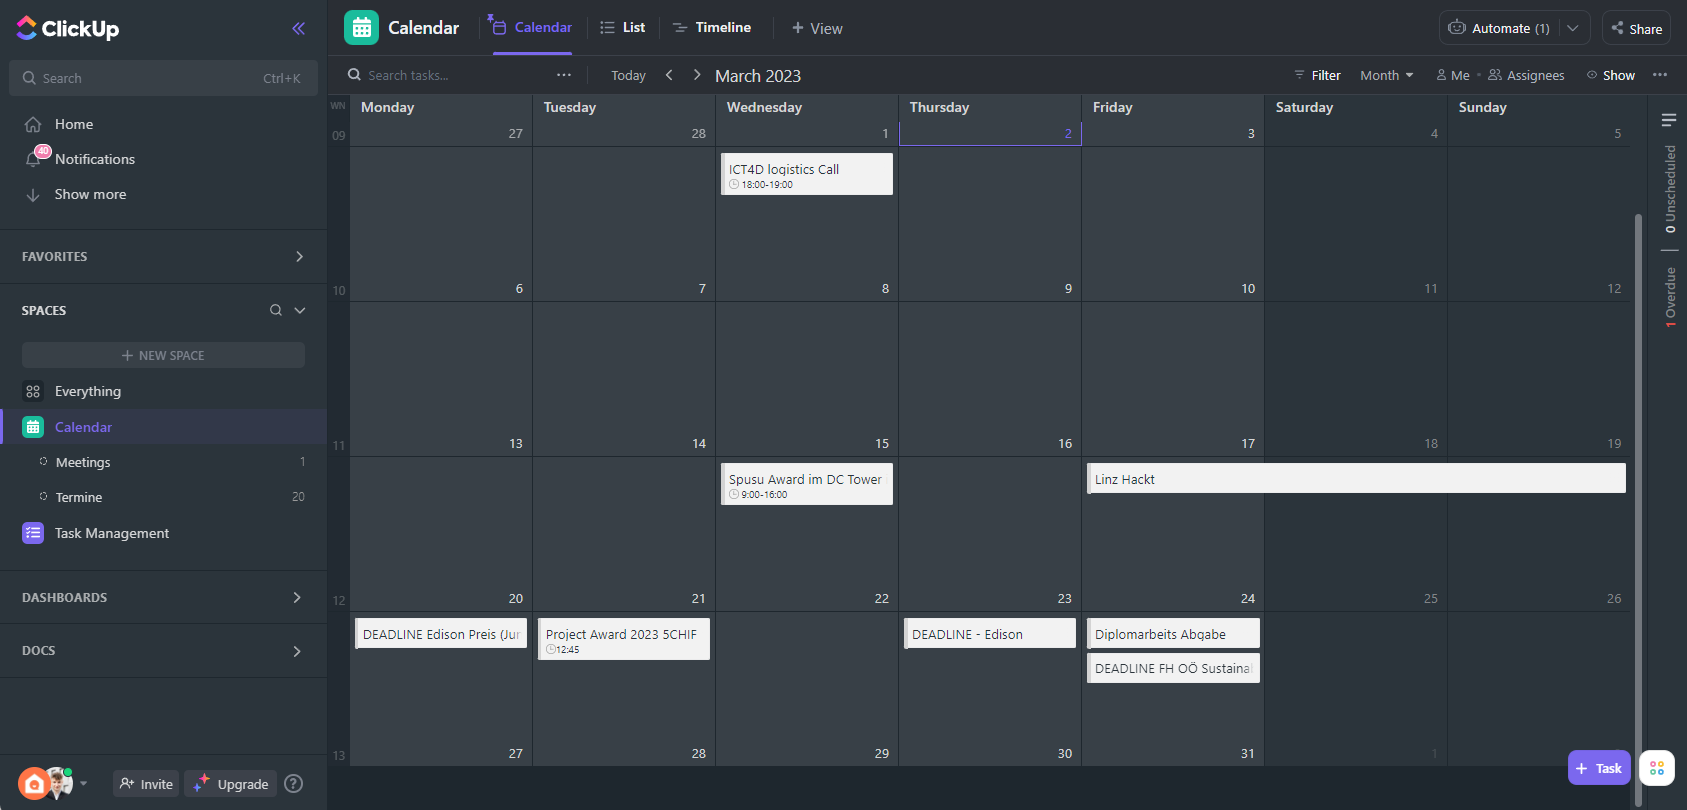
\includegraphics[width=1\textwidth]{./pics/clickup-calender-view.png}

In unserer Diplomarbeit haben wir viele Mentoring-Sessions,
Meetings mit unserem Diplomarbeitbetreuer und weitere
Termine wie Wettbewerbe. Ohne eine geeignete Methode zur
Verwaltung all dieser Termine kann es schnell
unübersichtlich werden. Daher haben wir das Kalender-Feature
von ClickUp genutzt, um alle unsere Einträge abzubilden. Auf der Abbildung sieht man den ClickUp Kalender-View, wie wir ihn benutzt haben. Ein großer Vorteil dabei war, dass der Kalender automatisch
mit unseren persönlichen Kalendern synchronisiert wurde, wie
beispielsweise meinem Google Kalender. Dadurch haben wir nie
einen Termin verpasst, was insbesondere für mich als
Projektleiter sehr hilfreich war, da ich nicht jeden daran
erinnern musste, alle Termine in seinem Kalender
einzutragen.

Ein weiterer wichtiger Punkt ist das Task-Management in
unserem Projekt. Da ich schnell viele Aufgaben koordinieren
musste, war es sinnvoll, alle Aufgaben in einer simplen
To-Do-Liste abzubilden. Vor den Semesterferien haben wir
beispielsweise eine eigene Abteilung für Ferien-Tasks
erstellt, um einen Überblick über alle Aufgaben während der
Semesterferien zu haben. Obwohl wir die Tasks sehr nicht
aktiv genutzt haben, war es sehr praktisch, um den
Fortschritt zu überwachen und sicherzustellen, dass alles
rechtzeitig erledigt wurde.

Zusammenfassend war ClickUp eine große Bereicherung für unser Projektmanagement, da es uns viel Zeit bei der Verwaltung von Terminen und Aufgaben gespart hat. Auch die Benutzung als neuer User war sehr einfach, sodass wir uns nicht lange einlesen mussten. Besonders faszinierend ist, dass ClickUp sehr intuitiv ist und viele nützliche Features bietet.


